\section{Shape Description and Modelling}

\subsection{Extracting features from shapes represented by connected components}

Lets consider the borders and boundaries of a connected component.

\begin{quote}
    The borders of a connected components are the outermost components, connected to an inner 8/4 component.
\end{quote}

\noindent We can describe the shape by region and boundary. One way to describe region is by simply calculating the area. We can calculate the perimeter/boundary length of a shape using the following formulae:

\begin{equation}
    P(S) = \sum_{j}\sqrt{( x_{j} - x_{j-1} )^{2} + (  y_{j} - y_{j-1} )^{2}}
\end{equation}

This formulae counts the straight line (L2) distance between two adjacent boundary \textit{points}.

\subsubsection{Shape Metrics}

\textbf{Compactness }We can measure 'tightly packed' the pixels in a component are. Its often computer as the weighted ratio of area to perimeter squared:

\begin{equation}
    C(s) = \frac{4\pi A(s)}{(P(s))^{2}}
\end{equation}

\noindent\textbf{Centre of Mass} We can measure the centre of mass by taking the mean of the x and y pixels in the component. \\

\noindent\textbf{Irregularity / Dispersion} We measure how 'spread' the shape is.

\begin{align}
    I(s) = \frac{\pi max( ( x_{j} - \Bar{x}  )^{2} + ( y_{j} - \Bar{y}  )^{2}) }{A(s)} \\
    IR(s) = \frac{ max \sqrt{( ( x_{j} - \Bar{x}  )^{2} + ( y_{j} - \Bar{y}  )^{2})} }{ min \sqrt{( ( x_{j} - \Bar{x}  )^{2} + ( y_{j} - \Bar{y}  )^{2})} }
\end{align}

\subsection{Moments}

Moments describe the distribution of pixels in a shape. We can compute these for \textbf{any grey-level image}. For this purpose, lets focus on the moments of a connected component.

\noindent The standard two dimensional Cartesian moment of an image, with order \textit{p} and \textit{q} is defined as:

\begin{equation}
    m_{pq} = \sum_{x}\sum_{y}x^{p}y^{q} I(x,y)\Delta A
\end{equation}

\noindent In the case of a connected component this is simplified to:

\begin{equation}
    m_{pq} = \sum_{i}x_{i}^{p}y_{i}^{q} 
\end{equation}

Therefore the zero order of a connected component $m_{00}$ is just the area of the component. The centre of mass is (centroid):

\begin{align}
    \bar{x} = \frac{m_{10}}{m00} \\
    \bar{y} = \frac{m_{01}}{m_{00}}
\end{align}

\subsubsection{Central Moments}

Standard 2D moments can be used as shape descriptors, however they are not invariant to translation, rotation and scaling.
\\
\noindent \textbf{Central Moments} are computed about the centroid of the shape, and are translation invariant:

\begin{equation}
    \mu_{pq} = \sum_{i} (x_{i} - \bar{x})^{p} (y_{i} - \bar{y})^{q}
\end{equation}

\noindent $\mu_{01}$ and $\mu_{10}$ are always 0, so have no descriptive power.

\noindent\textbf{Normalised Central Moments} are both scale and translation invariant:

\begin{equation}
    \eta_{pq} = \frac{\mu_{pq}}{\mu_{00}^{\frac{(p+q)}{2}}+1}
\end{equation}

\noindent\textbf{Hu Moments}

\noindent There exist 7 translation, scale and rotation invariant moments:

\begin{align*}
    M1 &= \eta_{20} +\eta_{02} \\
    M2 &= ( \eta_{20} - \eta_{02} )^{2} + 4\eta_{11}^2 \\
    M3 &= (\eta_{20}-3\eta_{12})^2 + (3\eta_{21}-\eta_{03})^2 \\
    M4 &= (\eta_{30} + \eta_{12})^2 + (\eta_{21}+\eta_{03})^2 \\
    M5 &= (\eta_{30}-3\eta_{12}) (\eta_{30}+\eta_{12}) \times ((\eta_{30}+\eta_{12} )^2 - 3( \eta_{21}+\eta_{03} )^2)  \\ &+ (3\eta_{21}-\eta_{03})(\eta_{21}+\eta_{03})(3(\eta_{30}+\eta_{12})^2 - (\eta_{21}+\eta_{03})^2) \\
    M6 &= (\eta_{20}-\eta_{02}) ((\eta_{30} + \eta_{12})^2 - (\eta_{21}+\eta_{03})^2) + 4\eta_{11}(\eta_{30}+\eta_{12})(\eta_{21}+\eta_{03}) \\
    M7 &= (3\eta_{21}-\eta_{03})(\eta_{30}+\eta_{12})( (\eta_{30}+\eta_{12})^2 - 3(\eta_{21}+\eta_{03})^2) \\ &+ (3\eta_{12}-\eta_{30})(\eta_{21}+\eta_{03})(3(\eta_{12}+\eta_{30})^2 - (\eta_{21}+\eta_{03})^2)
\end{align*}

\subsection{Chain Codes}
Simple way of encoding boundaries: We walk around the boundary and encode the direction you take, on each step, as a number. We then shift the code so it froms the smallest possible integer value. This is to make it invariant to the starting point.

\begin{figure}[!ht]
    \centering
    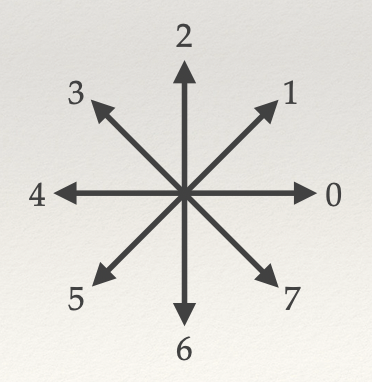
\includegraphics[scale=0.5]{Images/Chain.png}
    \caption{Directions}
    \label{fig:chain}
\end{figure}

Given a starting point, we refer to \ref{fig:chain} and go around the edges, and note the direction. We then sort the directions we took in ascending order.

\subsubsection{Chain Code Invariance}

We can make this \textbf{rotation invariant}, by encoding the differences in direction rather than absolute values. We can make this \textbf{scale invariant}, by resmapling the component to a fixed size.

\subsection{Active Shape Models and Constrained Local Models}

We can extend a Point Distribution Model by also learning local appearance around each point. This is used as an image template such as facial landmark...


